\section{Introduction}


\begin{frame}

  % Application pictures
\end{frame}

\begin{frame}{Text Generation}

  \[ \argmax_{y_{1:T}} f(y_{1:T} ; x, \theta)\]

\end{frame}

\begin{frame}{Natural Language Processing, 2009}

  % Picture
  \begin{tikzpicture}
    \node{};
  \end{tikzpicture}

\end{frame}

\begin{frame}{Natural Language Processing, 2019}

  % Picture
  \begin{tikzpicture}
    \node{};
  \end{tikzpicture}

\end{frame}

\begin{frame}{Performance}

\end{frame}


\begin{frame}

\end{frame}

\begin{frame}{Central}
  % Picture
  \begin{tikzpicture}
    \node{};
  \end{tikzpicture}
\end{frame}


\begin{frame}{My Research}{}
  % Picture
  \research{\cite{Deng2016}}


  \begin{tikzpicture}
    \node{};
  \end{tikzpicture}
\end{frame}


\begin{frame}{My Research}{}
  % Pictured






  \begin{center}
  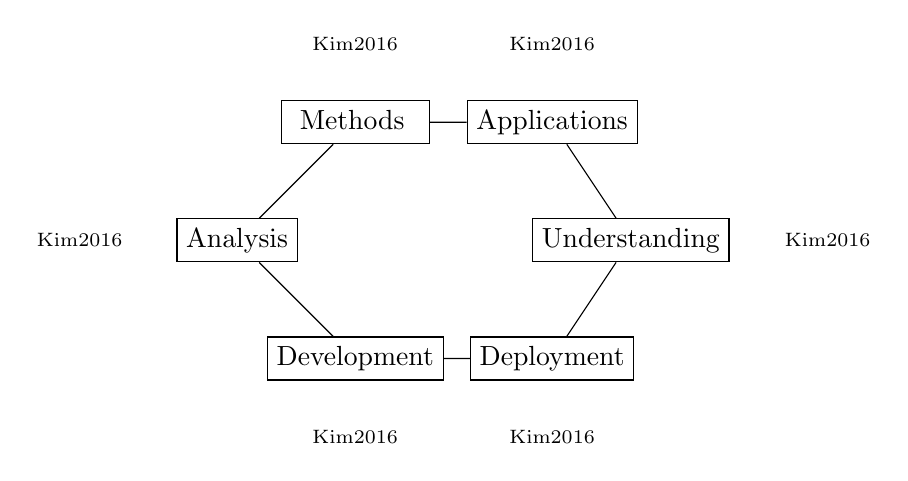
\begin{tikzpicture}

    \node at (-35mm, 15mm) {
      \scriptsize
      \citet{Kim2016}
      };
    \node[draw] (ana) at (-15mm, 15mm) {Analysis};
    \node[draw] (meth) at (0mm, 30mm) {\ Methods\phantom{p}};
    \node at (0mm, 40mm) {
      \scriptsize
      \citet{Kim2016}
      };

    \node[draw] (app) at (25mm, 30mm) {Applications};
    \node at (25mm, 40mm) {
      \scriptsize
      \citet{Kim2016}
      };



    \node[draw] (und) at (35mm, 15mm) {Understanding};


    \node at (60mm, 15mm) {
      \scriptsize
      \citet{Kim2016}
      };


    \node[draw] (dep) at (25mm, 0mm){Deployment};

    \node at (25mm, -10mm) {
      \scriptsize
      \citet{Kim2016}
      };

    \node[draw] (imp) at (0, 0) {Development};

      \node at (0mm, -10mm) {
      \scriptsize
      \citet{Kim2016}
      };


    \draw (ana) -- (meth) --(app) -- (und) -- (dep) -- (imp) -- (ana);

  \end{tikzpicture}
  \end{center}
\end{frame}

